\subsection{Generación de señalamiento paso a paso}
	
	Inicialmente, el RNA ejecuta el Algoritmo \ref{alg:graph_network} (ver Sección \ref{sec:grafos}) para detectar todos los \textit{netElements}, sus coordenadas iniciales y finales en la topología, y el sentido en el que fueron definidas. Al concluir el Algoritmo \ref{alg:graph_network}, el RNA ejecuta el Algoritmo \ref{alg:connectedness} (ver Sección \ref{sec:grafos}) para analizar la conexidad de la red. El resultado obtenido se muestra en el Código \ref{lst:EJ1_1}, donde se describen las coordenadas de cada \textit{netElement} y se confirma que la red es conexa.
	
	\begin{lstlisting}[language = {}, caption = Detección de \textit{netElements} por parte del RNA , label = {lst:EJ1_1}]
	###### Starting Railway Network Analyzer #####
	Reading .railML file
	Creating railML object
	Analysing railML object
	Analysing graph
	ne1 [810, 150] [1320, 150] >>
	ne2 [2970, 0] [2460, 0] <<
	ne8 [1320, 150] [1800, 150] >>
	ne9 [1320, 150] [1530, 360] >>
	ne12 [2460, 0] [1950, 0] <<
	ne13 [2460, 0] [810, -180] <<
	ne14 [1530, 360] [2970, 360] >>
	ne15 [1530, 360] [2970, 570] >>
	ne22 [1800, 150] [2970, 150] >>
	ne23 [1950, 0] [810, 0] <<
	ne24 [1800, 150] [1950, 0] >>
	The network is connected
	\end{lstlisting}
	
	Por ejemplo, el \textit{netElement} ne1 inicia en la coordenada (810;150) y finaliza en la coordenada (1320;150). El símbolo $>>$ indica que ne1 se encuentra definido de izquierda a derecha, ya que la componente x de la coordenada final es mayor a la de la coordenada inicial, teniendo la misma componente y. Además, se puede comprobar que la lista obtenida en consistente con la Figura \ref{fig:EJ1_2}. Por ejemplo, ne1, ne8 y ne9 comparten la coordenada (1320;150), que coincide con la coordenada del cambio de vías Sw04.
	
	A continuación, el RNA detectará la infraestructura ferroviaria, las curvas peligrosas y los puntos medios de los netElements que el RNA considera demasiado largos. El análisis de la infraestructura se detalla en la Sección \ref{sec:bufferstop}, Sección \ref{sec:detectors}, Sección \ref{sec:platform} y Sección \ref{sec:crossing}, mientras que la detección de curvas y puntos medios se detalla en la Sección \ref{sec:tracks}. El RNA ejecuta el Algoritmo \ref{alg:switches_1}, Algoritmo \ref{alg:switches_2} y Algoritmo \ref{alg:switches_3} para confirmar la detección de cambios de vías simples, dobles y en tijeras. El resultado de este proceso se puede visualizar en el Código \ref{lst:EJ1_2}.
	
	\begin{lstlisting}[language = {}, caption = Detección de puntos críticos por parte del RNA , label = {lst:EJ1_2}]
	Analysing infrastructure --> Infrastructure.RNA
	Detecting Danger --> Safe_points.RNA
	ne1 has a Middle point @ [1065.0, 150]
	ne2 has a Middle point @ [2715.0, 0]
	ne8 has a Middle point @ [1560.0, 150]
	ne12 has a Middle point @ [2205.0, 0]
	ne13 has a Platform[plf75] @ [1564, 180]
	ne13 has a LevelCrossing[lcr74] @ [1362, 180]
	ne13 has a Curve(2 lines) @ [[2280, -180]]
	ne14 has a Platform[plf68] @ [2490, -360]
	ne14 has a LevelCrossing[lcr69] @ [1945, -360]
	ne15 has a Curve(2 lines) @ [[1740, 570]]
	ne22 has a RailJoint[J15] @ [2452, 150]
	ne23 has a RailJoint[J14] @ [1284, 0]
	\end{lstlisting}
	
	Esta información es exportada por el RNA, con mayor detalle, en el archivo Infrastructure.RNA \ref{lst:EJ1_4} que resume cada elemento ferroviario asociado a su respectivo \textit{netElement}.
	
	\begin{lstlisting}[language = {}, caption = Infrastructure.RNA, label = {lst:EJ1_4}]
Nodes: 11|Switches: 5|Signals: 0|Detectors: 2|Ends: 7|Barriers: 2
Node ne1:
	Track = track1
	Neighbours = 2 -> ['ne8', 'ne9']
	Switches -> Sw04
		ContinueCourse -> right -> ne8
		BranchCourse -> left -> ne9
Node ne2:
	Track = track7
	Neighbours = 2 -> ['ne12', 'ne13']
	Switches -> Sw06
	ContinueCourse -> right -> ne12
	BranchCourse -> left -> ne13
Node ne8:
	Track = track2
	Neighbours = 4 -> ['ne1', 'ne9', 'ne22', 'ne24']
	Switches -> Sw12
		ContinueCourse -> left -> ne22
		BranchCourse -> right -> ne24
Node ne9:
	Track = track3
	Neighbours = 4 -> ['ne1', 'ne8', 'ne14', 'ne15']
	Switches -> Sw07
		ContinueCourse -> left -> ne15
		BranchCourse -> right -> ne14
Node ne12:
	Track = track8
	Neighbours = 4 -> ['ne2', 'ne13', 'ne23', 'ne24']
	Switches -> Sw13
		ContinueCourse -> left -> ne23
		BranchCourse -> right -> ne24
Node ne13:
	Track = track9
	Type = BufferStop -> ['bus56']
	Neighbours = 2 -> ['ne2', 'ne12']
	Level crossing -> lcr74
		Protection -> true | Barriers -> none | Lights -> none Acoustic -> none
		Position -> [1317, 180] | Coordinate: 0.7059
Node ne14:
	Track = track4
	Type = BufferStop -> ['bus10']
	Neighbours = 2 -> ['ne9', 'ne15']
	Level crossing -> lcr69
		Protection -> true | Barriers -> none | Lights -> none Acoustic -> none
		Position -> [1990, -360] | Coordinate: 0.3197
Node ne15:
	Track = track10
	Type = BufferStop -> ['bus59']
	Neighbours = 2 -> ['ne9', 'ne14']
Node ne22:
	Track = track6
	TrainDetectionElements -> tde78
	Type -> insulatedRailJoint
	Neighbours = 2 -> ['ne8', 'ne24']
Node ne23:
	Track = track5
	TrainDetectionElements -> tde77
	Type -> insulatedRailJoint
	Neighbours = 2 -> ['ne12', 'ne24']
Node ne24:
	Track = track11
	Neighbours = 4 -> ['ne8', 'ne12', 'ne22', 'ne23']
	\end{lstlisting}	
	
	La información de la infraestructura es utilizada por el RNA para detectar los puntos críticos de la red, es decir, las zonas donde es recomendable colocar una señal, según el sentido de circulación que se desee. El resultado es exportado al archivo SafePoints.RNA (Código \ref{lst:EJ1_5}). En el caso de que un mismo \textit{netElement} tenga más de un punto crítico para el mismo sentido, el RNA tomará el más cercano al elemento a proteger. El criterio de selección de puntos críticos se aplica para cada elemento ferroviario detectado, cada curva y cada cambio de vías y fue explicado en las secciones correspondientes ya mencionadas.
	
	\begin{lstlisting}[language = {}, caption = SafePoints.RNA, label = {lst:EJ1_5}]
ne1:
	Next: [[1065.0, 150]]
	Prev: [[1065.0, 150]]
ne2:
	Next: [[2715.0, 0]]
	Prev: [[2715.0, 0]]
ne8:
	Next: [[1560.0, 150]]
	Prev: [[1560.0, 150]]
ne12:
	Next: [[2205.0, 0]]
	Prev: [[2205.0, 0]]
ne13:
	Next: [[1162, 180], [2180.0, -180]]
	Prev: [[1764, 180]]
ne14:
	Next: [[2290, -360], [1745, -360]]
	Prev: [[2690, -360], [2145, -360]]
ne15:
	Prev: [[1840.0, 570]]
ne22:
	Next: [[2352.0, 150]]
	Prev: [[2552.0, 150]]
ne23:
	Next: [[1184.0, 0]]
	Prev: [[1384.0, 0]]
	\end{lstlisting}
	
	Una vez que el RNA detectó cada punto crítico de la red ferroviaria, procede a generar el señalamiento. El orden en que se procesan los elementos ferroviarios no impacta en el resultado final, pero para poder describirlo de forma ordenada se iniciará generando el señalamiento para proteger los finales de vías, las junturas entre rieles, las plataformas (explicado en la Sección \ref{sec:sig_platform}), los cruces de vía (explicado en la Sección \ref{sec:sig_levelcrossing}) y los cambios de vías (explicado en la Sección \ref{sec:signal_switches}). Luego se procederá a mostrar el señalamiento completo antes y después de la simplificación de señales (explicado en la Sección \label{sec:simplificacion}). 
	
	
	Tal cómo se explicó en la Sección \ref{sec:sig_border}, el RNA aplica el Algoritmo \ref{alg:lineBorder} y el Algoritmo \ref{alg:bufferStop} para generar las señales para proteger los finales de vías relativos y absolutos. Estas señales son ilustradas en la Figura \ref{fig:EJ1_3}.
	
	\begin{figure}[H]
		\centering
		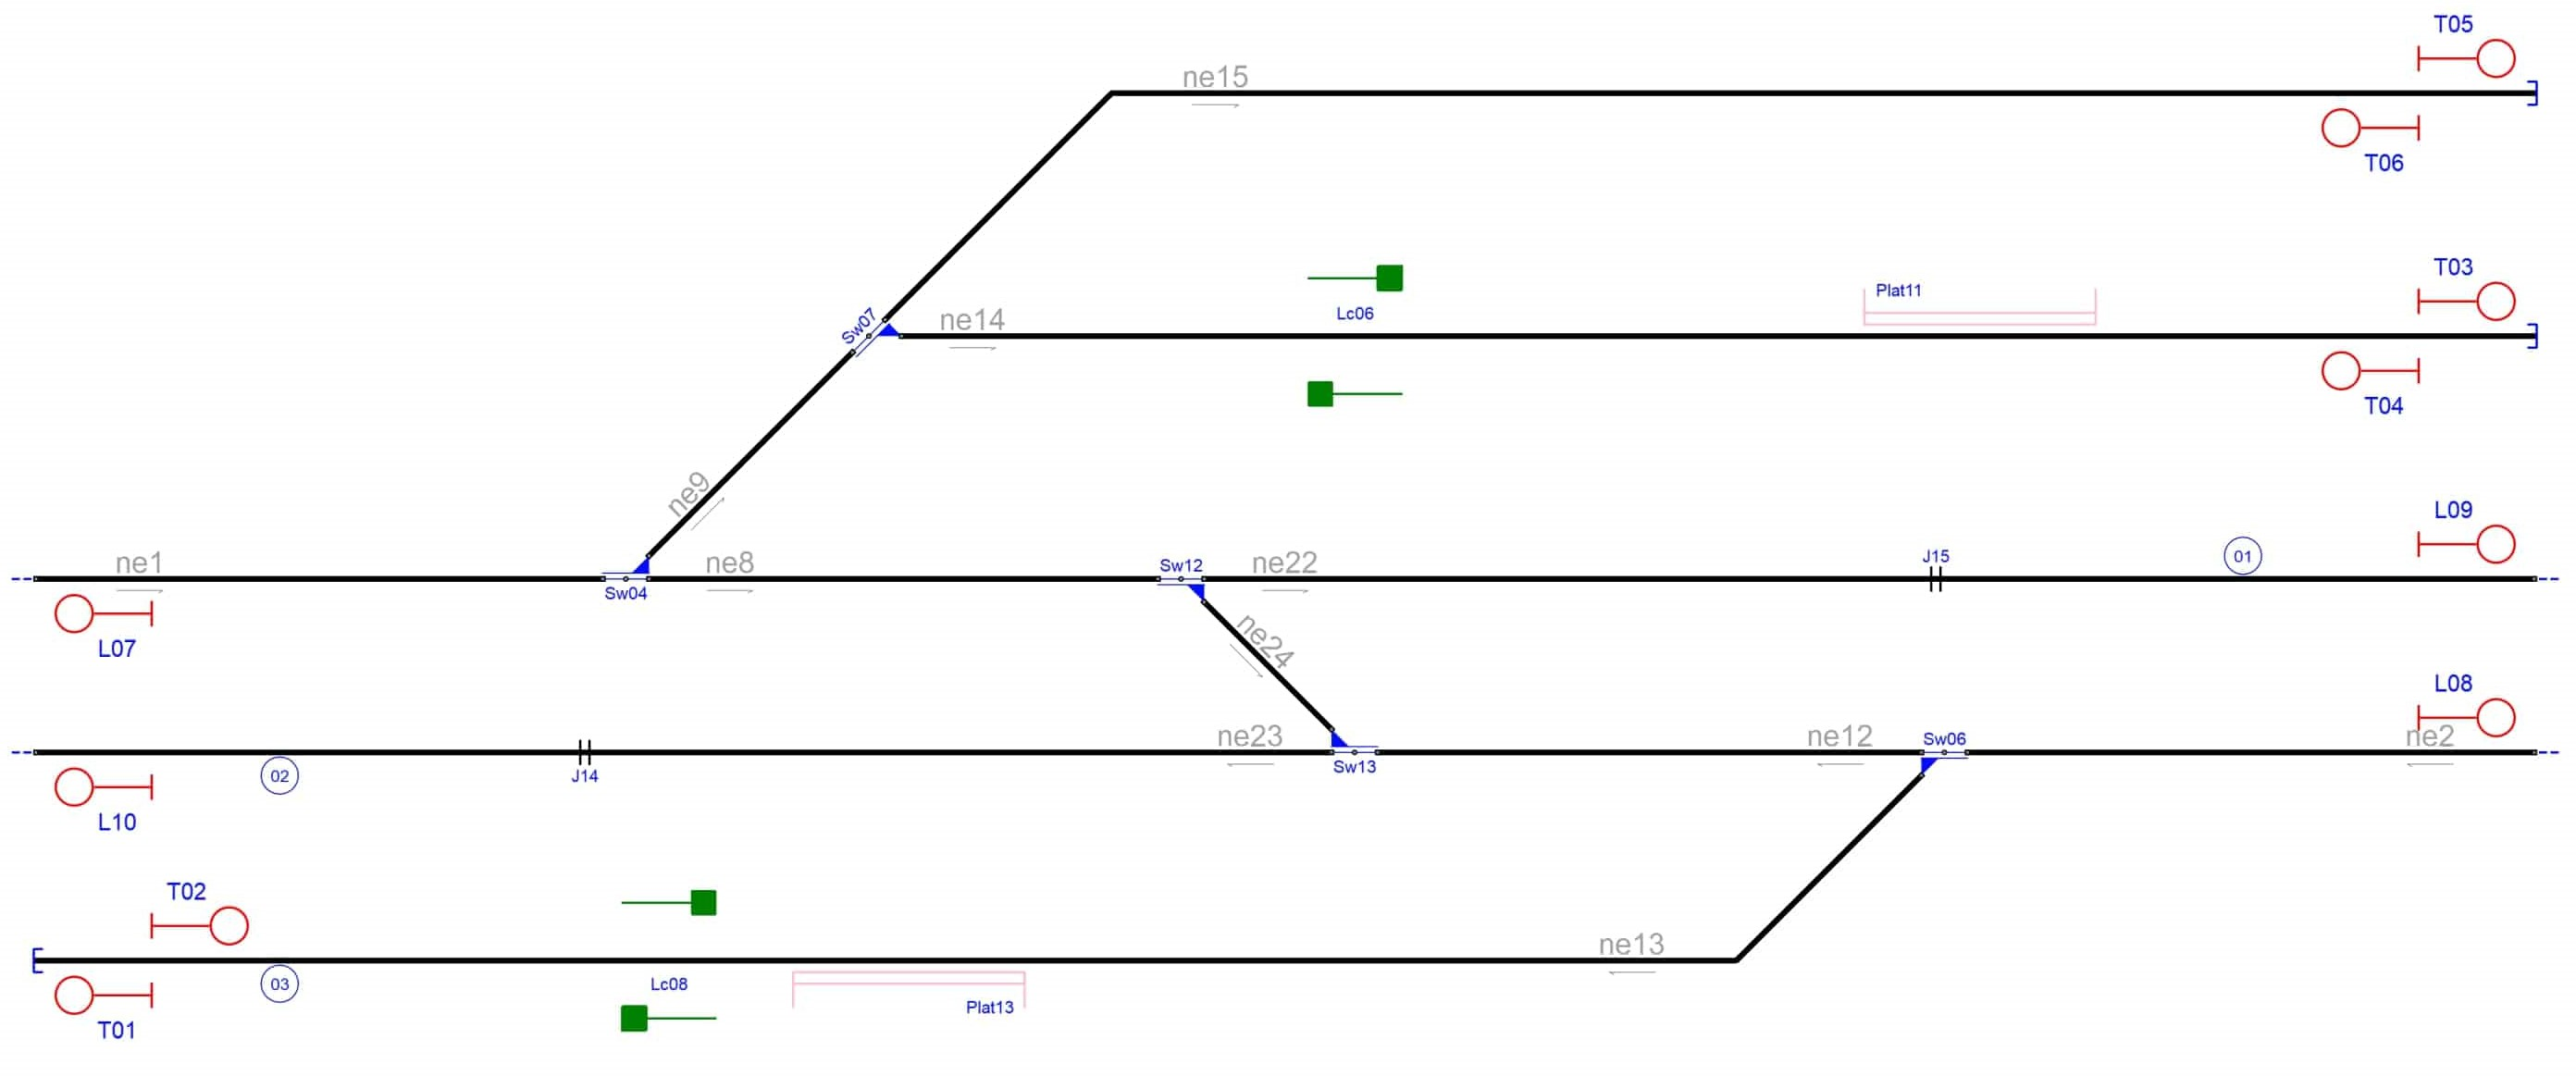
\includegraphics[width=1\textwidth]{resultados-obtenidos/ejemplo1/images/1_step1.png}
		\centering\caption{Señalamiento generado por el RNA para proteger el fin de vía.}
		\label{fig:EJ1_3}
	\end{figure}
	
	Los finales de vías absolutos son protegidos por las señales de parada T01, T03, T05 y las señales de partida son T02, T04 y T06. A su vez, los finales de vías relativos poseen las señales de parada L07, L08, L09 y L10, cercanos al límite del externo del \textit{netElement} al que pertenecen.
	
	La Figura \ref{fig:EJ1_4} ilustra la generación de señales destinadas a proteger las junturas entre los rieles. Estas señales se obtuvieron al aplicar el Algoritmo \ref{alg:RJ}, tal como fue explicado en la Sección \ref{sec:sig_joint}. Las señales generadas son J11, J12, J13 y J14, indicadas en color rojo. De no existir junturas que proteger, el RNA salteará este paso.
	
	\begin{figure}[H]
		\centering
		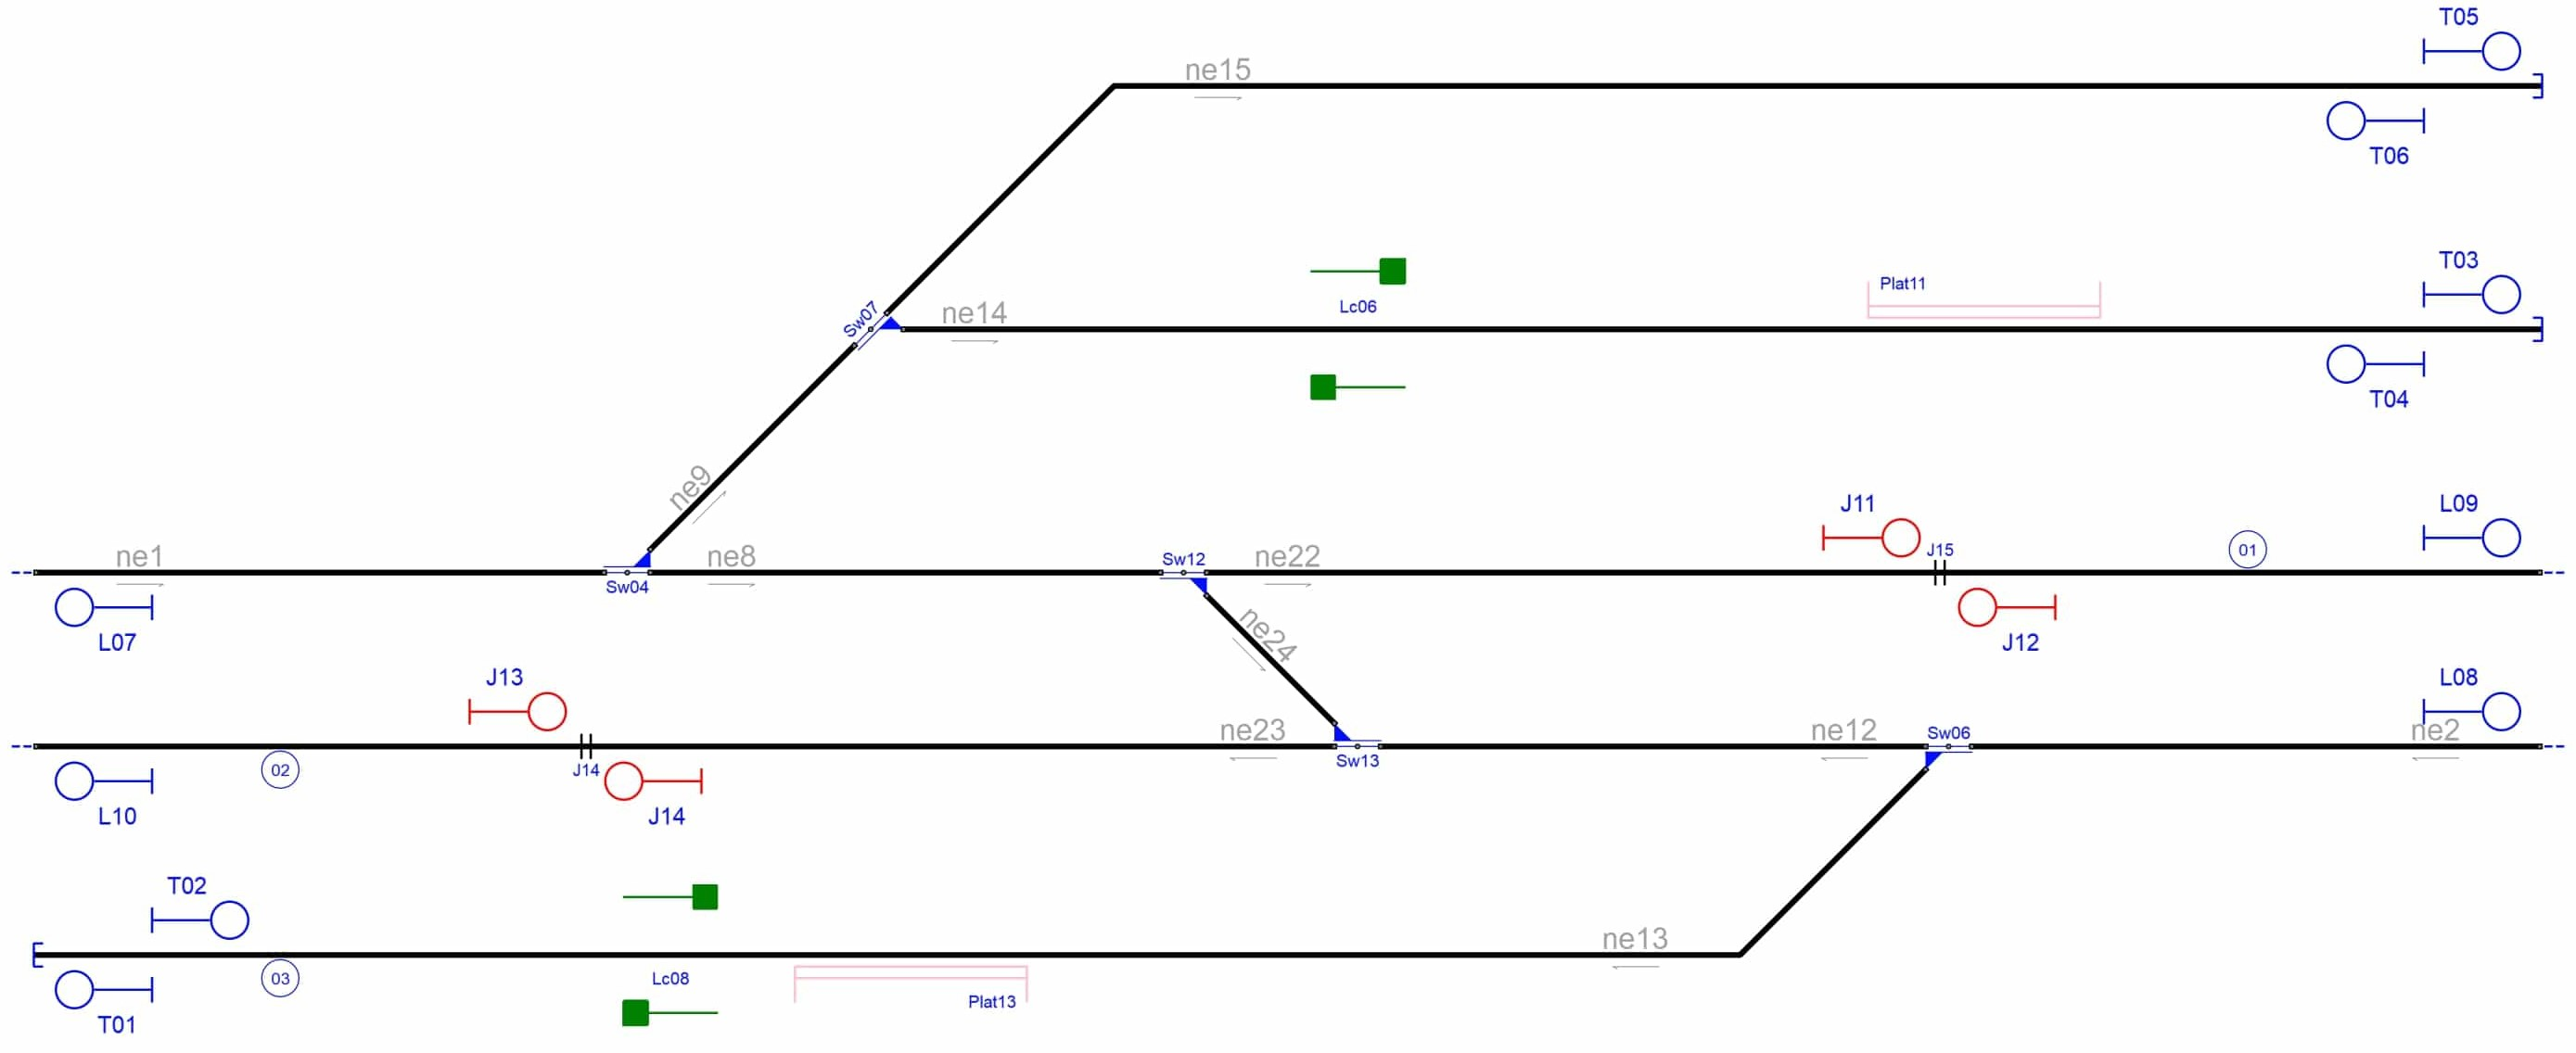
\includegraphics[width=1\textwidth]{resultados-obtenidos/ejemplo1/images/1_step2.png}
		\centering\caption{Señalamiento generado por el RNA para proteger las junturas.}
		\label{fig:EJ1_4}
	\end{figure}
	
	Al generar el señalamiento para proteger la infraestructura, tal como se explicó en la Sección \ref{sec:horizontal}, el Algoritmo \ref{alg:horizontal} simplificará las señales entre dos elementos ferroviarios si no existe espacio suficiente entre ellos, tal como sucede con los elementos levelCrossing8 y Platform13. El señalamiento generado para proteger las plataformas y los cruces de vía, producto de aplicar el Algoritmo \ref{alg:PTF} y el Algoritmo \ref{alg:LC}, respectivamente, se ilustra en rojo en la Figura \ref{fig:EJ1_5}. Las señales generadas para proteger las plataformas son las señales de partida P18, P19 y P20, mientras que las señales que protegen los cruces de vía son las señales X15, X16 y X17.
		
	\begin{figure}[H]
		\centering
		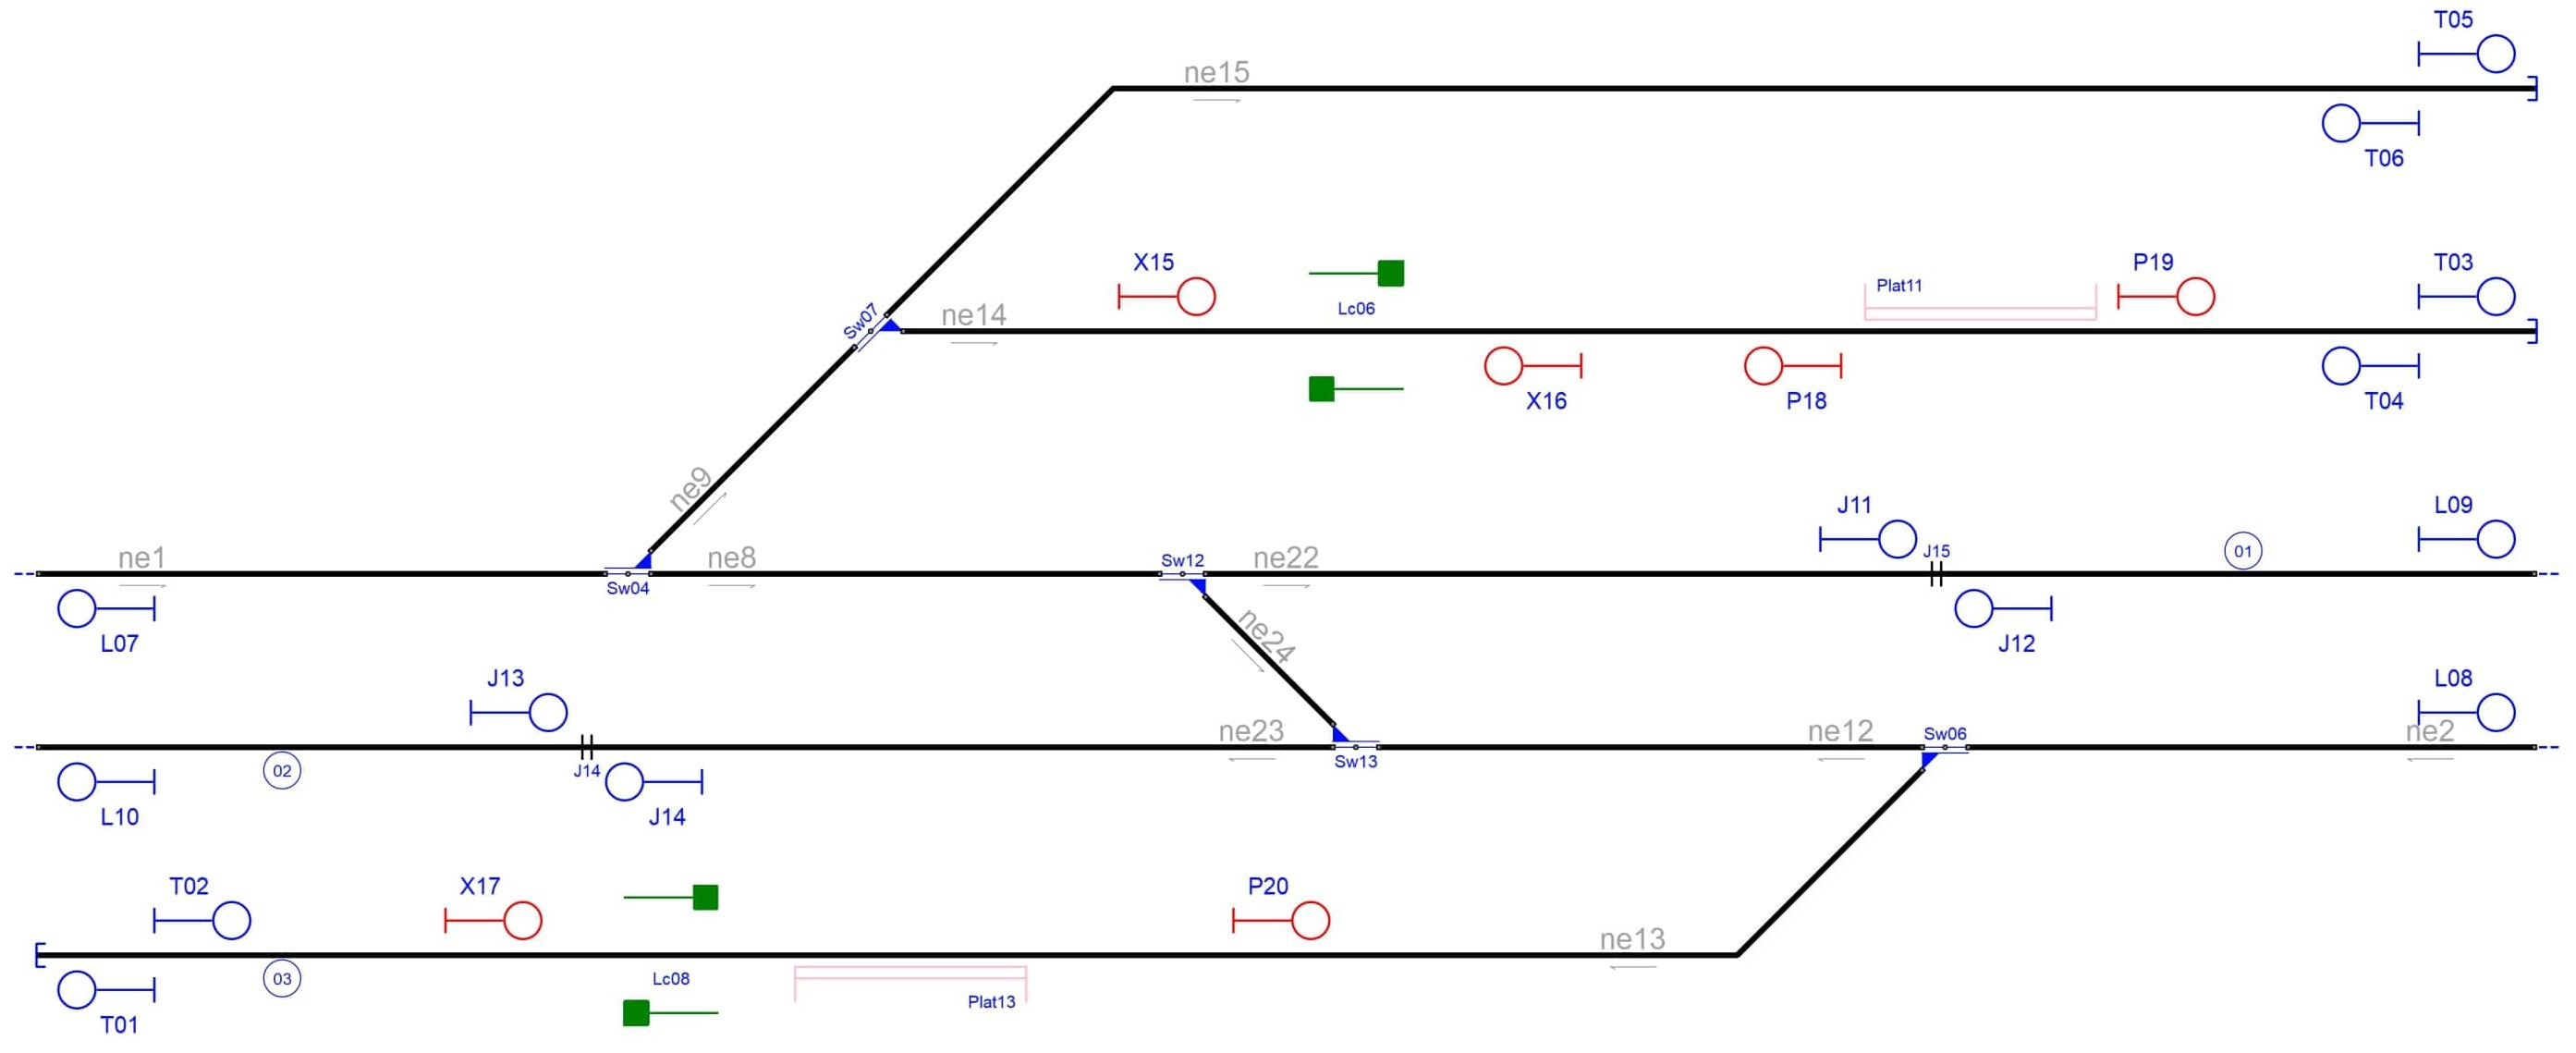
\includegraphics[width=1\textwidth]{resultados-obtenidos/ejemplo1/images/1_step3.png}
		\centering\caption{Señalamiento generado por el RNA para proteger plataformas y cruces de vía.}
		\label{fig:EJ1_5}
	\end{figure}
	
	Al aplicar el Algoritmo \ref{alg:SW} de generación de señalamiento para cambios de vías, tal como fue explicado en la Sección \label{sec:signal_switches}, se generan las señales S22, C21, H23 y H24 para proteger el cambio de vías Sw04; las señales S27, C25, B26 y H28 para proteger el cambio de vías Sw06; las señales C29 y B30 para proteger el cambio de vías Sw07; las señales S32, C31 y H33 para proteger el cambio de vías Sw12 y las señales S35, C34 y H36 para proteger el cambio de vías Sw13. Estas señales se encuentran resaltadas en rojo en la Figura \ref{fig:EJ1_6}.
	
	\begin{figure}[H]
		\centering
		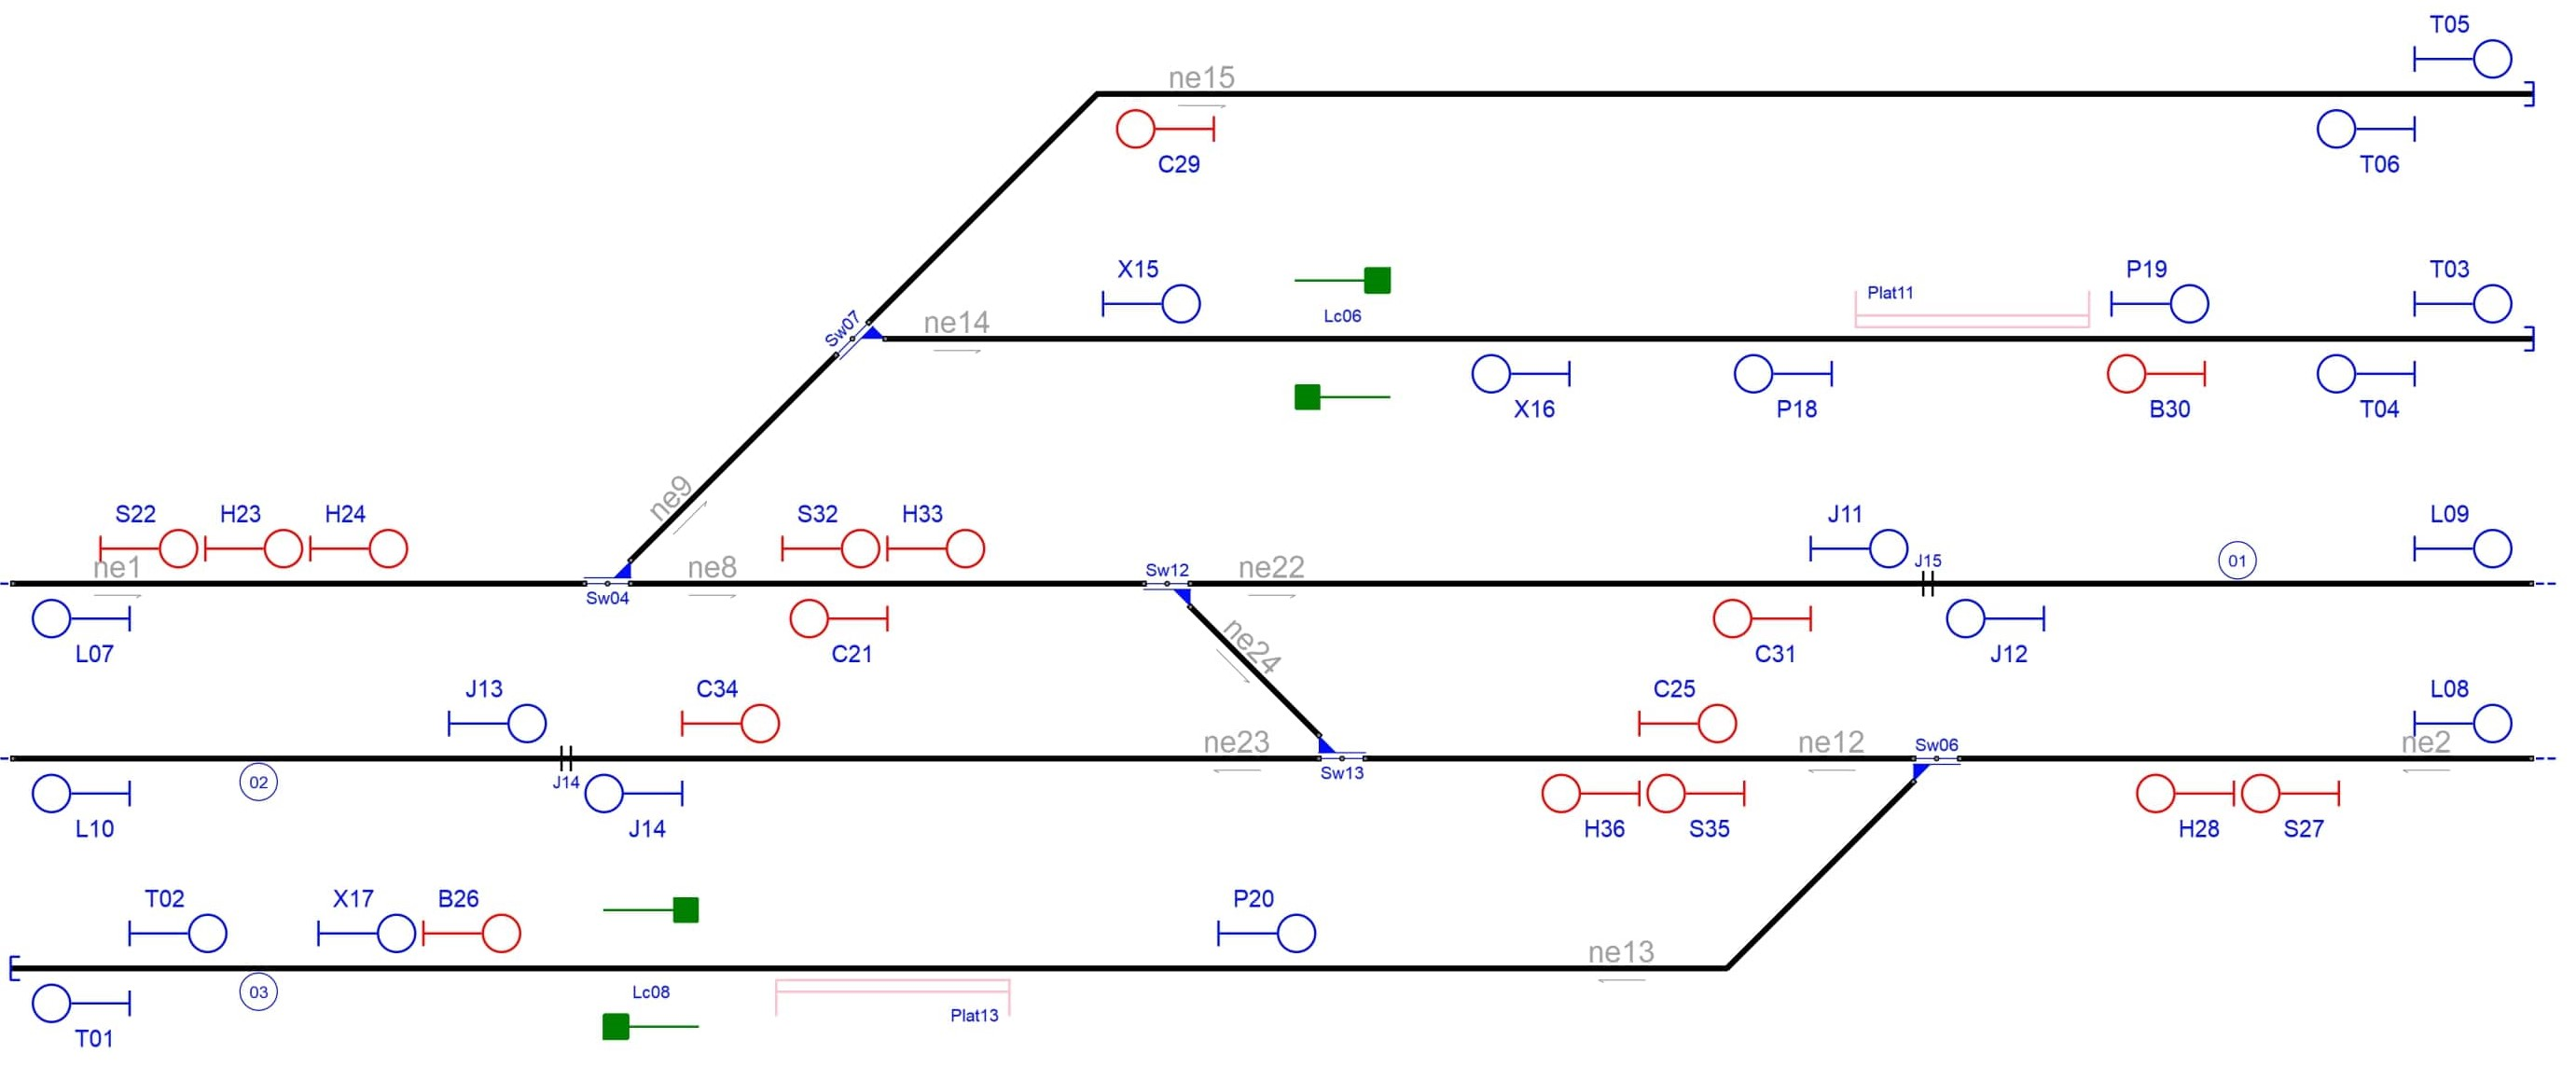
\includegraphics[width=1\textwidth]{resultados-obtenidos/ejemplo1/images/1_step4.png}
		\centering\caption{Señalamiento generado por el RNA para proteger los cambios de vías.}
		\label{fig:EJ1_6}
	\end{figure}
	
	Una vez obtenido todo el señalamiento, el RNA procede a simplificar las señales redundantes, repetidas o cuyas funciones o ubicaciones se superponen entre sí. El proceso de simplificación de señales fue explicado en la Sección \ref{sec:simplificacion}. El Algoritmo \ref{alg:vertical} de herencia vertical fue aplicado en las señales B entre los cambios de vías Sw12 y Sw13, desplazando las señales hasta convertirlas en las señales H33 y H36 respectivamente. Análogamente, las señales C y S del \textit{netElement} se convirtieron en las señales H23 y H24 respectivamente.
	
	Las señales simplificadas al aplicar el Algoritmo \ref{alg:horizontal} de herencia horizontal son: X17, P18, P19, B26, B30, C31 y C34. Las señales X17 y B26 fueron eliminadas por su cercanía con la señal T02, con la cual comparten dirección y sentido. Lo mismo ocurre entre el par de señales P18/B30 y la señal T04; entre las señales P19 y T03; entre las señales C31 y J12; y entre las señales C34 y J13. En todos los casos, se aplicó el Algoritmo \ref{alg:horizontal}, diseñado para agrupar objetos cercanos como un único objeto, y así generar el señalamiento acorde a los elementos contenidos en cada extremo del nuevo elemento contenedor.
	
	Finalmente, las señales son simplificadas aplicando el Algoritmo \ref{alg:reduction} de eliminación por prioridad de señales. El resultado de este proceso es detallado en el Código \ref{lst:EJ1_3}.
	
	\begin{lstlisting}[language = {}, caption = Reducción de señalamiento por prioridad de señales, label = {lst:EJ1_3}]
	Reducing redundant signals
	removing sig17 for sig02
	removing sig26 for sig02
	removing sig19 for sig03
	removing sig30 for sig04
	removing sig31 for sig12
	removing sig34 for sig13
	removing sig18 for sig30
	\end{lstlisting}
	
	El resultado de la simplificación del señalamiento se ilustra en la Figura \ref{fig:EJ1_7}.
	
	\begin{figure}[H]
		\centering
		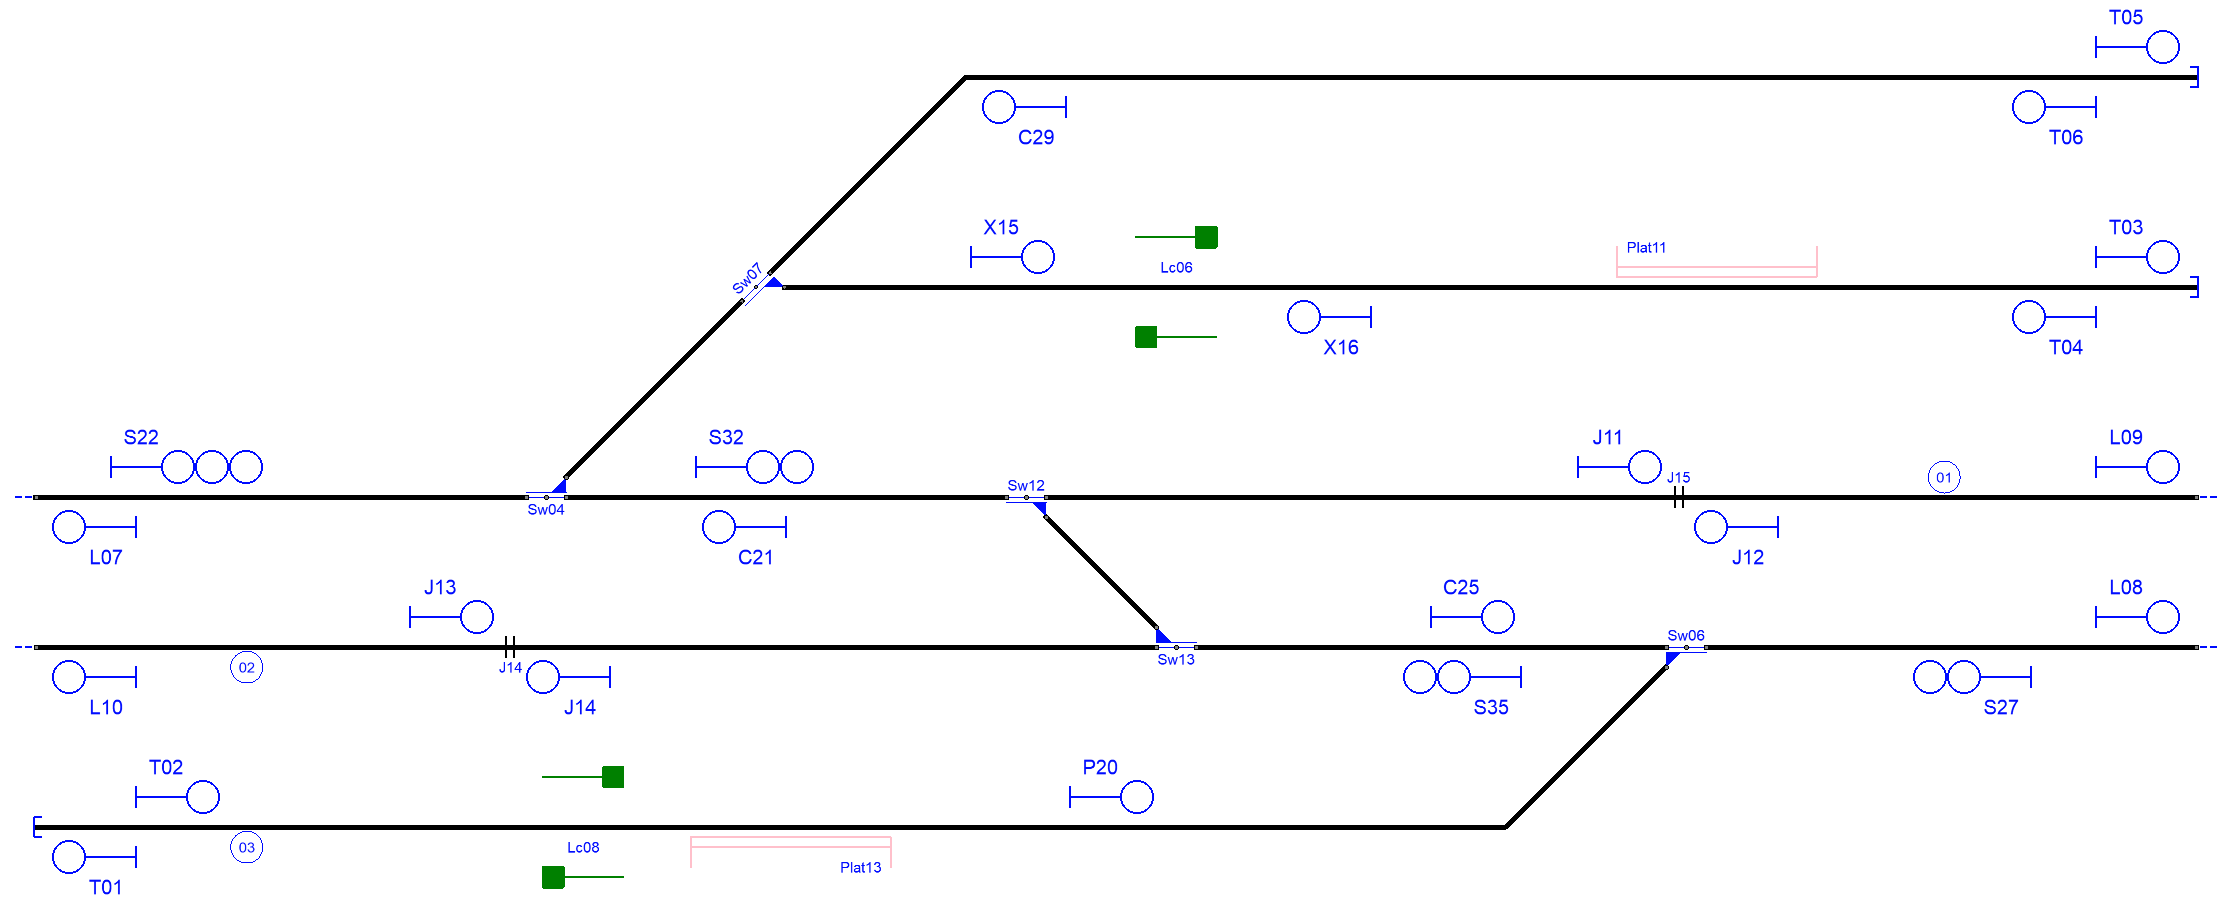
\includegraphics[width=1\textwidth]{resultados-obtenidos/ejemplo1/images/1_RNA.png}
		\centering\caption{Señalamiento generado y simplificado por el RNA.}
		\label{fig:EJ1_7}
	\end{figure}
	
	Además, toda la información del señalamiento generado es exportada por el RNA en el archivo Signalling.RNA (Código \ref{lst:EJ1_6}), que incluye información detallada de la posición, orientación, sentido, coordenada, nombre y tipo de señal.
		
	\begin{lstlisting}[language = {}, caption = Signalling.RNA, label = {lst:EJ1_6}]
T01 [T01] <<:
	From: ne13 | To: bus56_left
	Type: Stop | Direction: normal | AtTrack: left 
	Position: [910, 180] | Coordinate: 0.2055
T02 [T02] >>:
	From: ne13 | To: ne13_right
	Type: Stop | Direction: reverse | AtTrack: right 
	Position: [910, 180] | Coordinate: 0.2055
T03 [T03] >>:
	From: ne14 | To: bus10_right
	Type: Stop | Direction: normal | AtTrack: left 
	Position: [2870, -360] | Coordinate: 0.9305
T04 [T04] <<:
	From: ne14 | To: ne14_left
	Type: Stop | Direction: reverse | AtTrack: right 
	Position: [2870, -360] | Coordinate: 0.9305
T05 [T05] >>:
	From: ne15 | To: bus59_right
	Type: Stop | Direction: normal | AtTrack: left 
	Position: [2870, -570] | Coordinate: 0.9345
T06 [T06] <<:
	From: ne15 | To: ne15_left
	Type: Stop | Direction: reverse | AtTrack: right 
	Position: [2870, -570] | Coordinate: 0.9345
L07 [L07] <<:
	From: ne1 | To: oe40_left
	Type: Circulation | Direction: reverse | AtTrack: right 
	Position: [910, -150] | Coordinate: 0.1960
L08 [L08] >>:
	From: ne2 | To: oe42_right
	Type: Circulation | Direction: reverse | AtTrack: right 
	Position: [2870, 0] | Coordinate: 0.8039
L09 [L09] >>:
	From: ne22 | To: oe41_right
	Type: Circulation | Direction: normal | AtTrack: left 
	Position: [2870, -150] | Coordinate: 0.9145
J11 [J11] >>:
	From: ne22 | To: ne22_right
	Type: Circulation | Direction: normal | AtTrack: left 
	Position: [2352.0, -150] | Coordinate: 0.4717
J12 [J12] <<:
	From: ne22 | To: ne22_left
	Type: Circulation | Direction: reverse | AtTrack: right 
	Position: [2552.0, -150] | Coordinate: 0.6427
J13 [J13] >>:
	From: ne23 | To: ne23_right
	Type: Circulation | Direction: reverse | AtTrack: right 
	Position: [1184.0, 0] | Coordinate: 0.3280
J14 [J14] <<:
	From: ne23 | To: ne23_left
	Type: Circulation | Direction: normal | AtTrack: left 
	Position: [1384.0, 0] | Coordinate: 0.5035
X15 [X15] >>:
	From: ne14 | To: ne14_right
	Type: Circulation | Direction: normal | AtTrack: left 
	Position: [1745, 360] | Coordinate: 0.5218
X16 [X16] <<:
	From: ne14 | To: ne14_left
	Type: Circulation | Direction: reverse | AtTrack: right 
	Position: [2145, 360] | Coordinate: 0.6575
P20 [P20] >>:
	From: ne13 | To: ne13_right
	Type: Circulation | Direction: reverse | AtTrack: right 
	Position: [1844, -180] | Coordinate: 0.7824
C21 [C21] <<:
	From: ne8 | To: ne8_left
	Type: Circulation | Direction: reverse | AtTrack: right 
	Position: [1560.0, -150] | Coordinate: 0.5
S22 [S22] >>:
	From: ne1 | To: ne1_right
	Type: Circulation | Direction: normal | AtTrack: left 
	Position: [1065.0, -150] | Coordinate: 0.5
C25 [C25] >>:
	From: ne12 | To: ne12_right
	Type: Circulation | Direction: reverse | AtTrack: right 
	Position: [2205.0, 0] | Coordinate: 0.5
S27 [S27] <<:
	From: ne2 | To: ne2_left
	Type: Circulation | Direction: normal | AtTrack: left 
	Position: [2715.0, 0] | Coordinate: 0.5
C29 [C29] <<:
	From: ne15 | To: ne15_left
	Type: Manouver | Direction: reverse | AtTrack: right 
	Position: [1840.0, -570] | Coordinate: 0.2599
S32 [S32] >>:
	From: ne8 | To: ne8_right
	Type: Circulation | Direction: normal | AtTrack: left 
	Position: [1560.0, -150] | Coordinate: 0.5
S35 [S35] <<:
	From: ne12 | To: ne12_left
	Type: Circulation | Direction: normal | AtTrack: left 
	Position: [2205.0, 0] | Coordinate: 0.5
	\end{lstlisting}
	
	Al finalizar la generación del señalamiento, el RNA ejecuta el Algoritmo \ref{alg:routes}, explicado en la Sección \ref{sec:rutas}, para detectar todas las posibles rutas admitidas por la red para crear la tabla de enclavamientos. La cuál puede ser visualizada en el archivo Routes.RNA (Código \ref{lst:EJ1_7}). La misma detalla las señales de inicio y final, los \textit{netElements} abarcados por la ruta y cualquier infraestructura involucrada, incluyendo el estado que deben tener para que la ruta sea activada.
	
	\begin{lstlisting}[language = {}, caption = Routes.RNA, label = {lst:EJ1_7}]
route_1 [T02 >> P20]:
	Path: ['ne13']
	Platforms: ['Plat13']
	LevelCrossings: ['Lc08']
route_2 [T04 << X16]:
	Path: ['ne14']
	Platforms: ['Plat11']
route_3 [T06 << C29]:
	Path: ['ne15']
route_4 [J11 >> L09]:
	Path: ['ne22']
route_5 [J12 << C21]:
	Path: ['ne22', 'ne8']
	Switches: ['Sw12_N']
route_6 [J13 >> C25]:
	Path: ['ne23', 'ne12']
	Switches: ['Sw13_N']
route_7 [X15 >> T03]:
	Path: ['ne14']
	Platforms: ['Plat11']
	LevelCrossings: ['Lc06']
route_8 [X16 << L07]:
	Path: ['ne14', 'ne9', 'ne1']
	Switches: ['Sw04_R', 'Sw07_R']
	LevelCrossings: ['Lc06']
route_9 [P20 >> L08]:
	Path: ['ne13', 'ne2']
	Switches: ['Sw06_R']
route_10 [C21 << L07]:
	Path: ['ne8', 'ne1']
	Switches: ['Sw04_N']
route_11 [S22 >> S32]:
	Path: ['ne1', 'ne8']
	Switches: ['Sw04_N']
route_12 [S22 >> X15]:
	Path: ['ne1', 'ne9', 'ne14']
	Switches: ['Sw04_R', 'Sw07_R']
route_13 [S22 >> T05]:
	Path: ['ne1', 'ne9', 'ne15']
	Switches: ['Sw04_R', 'Sw07_N']
route_14 [C25 >> L08]:
	Path: ['ne12', 'ne2']
	Switches: ['Sw06_N']
route_15 [S27 << S35]:
	Path: ['ne2', 'ne12']
	Switches: ['Sw06_N']
route_16 [S27 << T01]:
	Path: ['ne2', 'ne13']
	Switches: ['Sw06_R']
	Platforms: ['Plat13']
	LevelCrossings: ['Lc08']
route_17 [C29 << L07]:
	Path: ['ne15', 'ne9', 'ne1']
	Switches: ['Sw04_R', 'Sw07_N']
route_18 [S32 >> J11]:
	Path: ['ne8', 'ne22']
	Switches: ['Sw12_N']
route_19 [S32 >> C25]:
	Path: ['ne8', 'ne24', 'ne12']
	Switches: ['Sw12_R', 'Sw13_R']
route_20 [S35 << J14]:
	Path: ['ne12', 'ne23']
	Switches: ['Sw13_N']
route_21 [S35 << C21]:
	Path: ['ne12', 'ne24', 'ne8']
	Switches: ['Sw12_R', 'Sw13_R']
	\end{lstlisting}	
		